% !TeX root = ../mythesis.tex
% !TeX encoding = UTF-8
% !TeX spellcheck = en_US

% \subsection{Motivation}
%% MOTIVATION %%

%- MOTIVATION/ClausalForm
%- MOTIVATION/Notation

%+ MOTIVATION/forwardSubsumption.tex

% \begin{example}[forward subsumption]
% 	\begin{gather*}
% 	S = \{ \TI{1}\mP(x,y), \TI{2}\lnot \mP(\ma,z)\} \cup \{\TI{3}\colG\mP(\ma,z') \}
% 	\tag*{\( \mcC_1 \) subsumes \( \mcC_3 \)}
% 	\\[0.7em]
% 	\infer[\{x\mapsto\ma,y\mapsto z\}]
% 	{\square}
% 	{\mP(x,y) & \lnot \mP(\ma,z)}
% 	\tag*{Resolution}
% 	\\[0.7em]
% 	S\bot = \{ \mP(\bot,\bot), {\colLo\lnot \mP(\ma,\bot), \mP(\ma,\bot)} \}
% 	\tag*{InstGen / SMT}
% 	\end{gather*}
% \end{example}

%+ MOTIVATION/goalEffectiveCalculus
%+ MOTIVATION/goalFastTermRetrieval
%+ MOTIVATION/goalSoundComplete


	% \begin{enumerate}
	% 	\item {Reduce} search space
	% 	\begin{itemize}
	% 		\item Ordered Resolution, Strategies, \ldots
	% 		\item \ldots with selection functions for clauses and literals
	% 	\end{itemize}
	% 	\item {Reduce} redundancy
	% 	\begin{itemize}
	% 		\item e.g.~discard clauses that are subsumed by other clauses
	% 		\item \ldots depending on the calculus
	% 	\end{itemize}
		% \item
		% Quickly find
		% \begin{itemize}
		% 	\item {variants} \hfill{\footnotesize variant removal}

		% 	\item {instances}   \hfill{\footnotesize backward subsumption}\\
		% 	\( \INST(s,t)\Leftrightarrow\exists\sigma\ s = t\sigma \)

		% 	\item {generalizations}  \hfill{\footnotesize forward subsumption}\\
		% 	\( \GNRL(s,t)\Leftrightarrow\exists\sigma\ s\sigma = t \)

		% 	\item {unifiable terms} \hfill{\footnotesize resolution, demodulation}\\
		% 	\( \UNIF(s,t)\Leftrightarrow\exists\sigma\ s\sigma = t\sigma \)

		% \end{itemize}

		% of a query term in a given set of terms.
	% \end{enumerate}




% \begin{tikzpicture}[scale = 1, transform shape, draw=black, fill=black, thick, sloped]

% \draw[->, ultra thick] (0,0) --
% node[pos=0, above] {\( F \)}
% (2,0);

% % outer rectangle
% \draw[rounded corners=-1.5mm] (1,3) rectangle (8.5,-3);
% % is F a theorem?
% \draw(2.4,2.7) node {\color{colN}Is \( F \) a theorem?};

% % SLIDE Is S satisfiable?
% \node[colG] (S) at (1.6,-2.7) {\scriptsize\( \lnot F \approx S \)};
% \node (S) at (2.5,0) {\( S \)};


% % SLIDE 2
% \draw[thin,dashed,draw=colO] (2.5,0) ellipse (0.4 and 1.2); % S

% % inner rectangle
% \draw[rounded corners=-1.5mm]  (1.5,-2.25) rectangle (8,2.25);
% % is S satisfiable?
% \draw (3.2,-1.9) node {\color{colN}Is \( \lnot F \) satisfiable?};

% % SLIDE unsatisfiable
% \draw[thin,dashed,draw=colO] (2.6,0) ellipse (0.6 and 1.44);  % S
% \draw[dashed, draw=colG, thick] decorate[decoration={snake}] {(1.4, 1) -- (8.2,0.6)};
% \draw[->, draw=colHi, ultra thick] (6.5,1.8) --
% node[pos=0,below] {unsatisfiable}
% node[pos=0.85, above] {theorem}
% (10,1.8) ;

% % SLIDE satisfiable
% \draw[thin,dashed,draw=colO] (2.8,0) ellipse (0.9 and 1.73);  % S
% \draw[dashed, draw=colG, thick]  decorate[decoration={snake}] { (1.4,-1)  --  (8.2,-0.6) };
% \draw[->,draw=colLo, ultra thick] (7,-1.3) --
% node[pos=0, below] {satisfiable}
% node[pos=0.75, above] {not a theorem} (11,-1.3) ;

% % SLIDE 5
% \draw[thin,dashed,draw=colO] (3.2,0) ellipse (1.35 and 2.07); % S
% \draw[->,draw=colNa, ultra thick] (7,0.15) --
% %	node[pos=0,above] {space out}
% node[pos=0,below] {time out}
% node[pos=0.85, above] {maybe} (10.5,0.15) ;
% \end{tikzpicture}

%%


%+ POSITION/Normalization
\begin{example}{Variable normalization}
	Variants of terms generate the same position strings
	\begin{itemize}
		\item if variable names are ignored
		\hfill \( \mf(y,z) \Rightarrow
		\ANGLES{\epsilon,\mf}
		\ANGLES{1,*}
		\ANGLES{2,*}
		 \)

		\item or normalized
		\hfill \( \mf(y,z) \Rightarrow
		\ANGLES{\epsilon,\mf}
		\ANGLES{1,x_1}
		\ANGLES{2,x_2} \)
		\\
		\hfill \( \mf(y,y) \Rightarrow
		\ANGLES{\epsilon,\mf}
		\ANGLES{1,x_1}
		\ANGLES{2,x_1}
		 \)
	\end{itemize}

	In the first case even non-variants of terms generate the same strings.
\end{example}


%+ POSITION/PositionStrings + Term traversals




%+ POSITION/Simplification


\subsection{Path Indexing}

%% PATH INDEXING %%

%+ PATH INDEXING/Build+Index
\begin{example}{Build}
	\def\TRIEWIDTH{4cm}
	\def\TEXTWIDTH{\textwidth-\TRIEWIDTH-2em}

	\begin{minipage}{\TEXTWIDTH}
		\(
		\TI{t_1}\,\mh(\mf(x,y)),
		\TI{t_2}\mh(\mf( x,\ma)),
		\TI{t_3}\mh(\mf(\ma,\ma))
		 \)
		\begin{align*}
		t_1 &\Rightarrow \{ \mh.1.\mf.1.{*},  \mh.1.\mf.2.{*} \} \\
		t_2 &\Rightarrow \{ \mh.1.\mf.1.{*},  \mh.1.\mf.2.\ma \} \\
		t_3 &\Rightarrow \{ \mh.1.\mf.1.\ma,  \mh.1.\mf.2 \ma \}
		\end{align*}
	\end{minipage}
%
	\begin{minipage}{\TRIEWIDTH}
	\begin{tikzpicture}[->,dotted]
%		\renewcommand{\PAUSE}{\pause}
%		\ORIGIN

\def\pyL{-0.2}
\def\pxL{0.05}

\PAUSE

\node (root) at (2.5,5) {.};
\node (h) at (2.5,4) {.};
\path (root) edge node {$\mh$} (h);

\PAUSE
\node (h1) at (2.5,3) {.};
\path (h) edge node {$1$} (h1);

\PAUSE
\node (h1f) at (1.5,2) {.};
\path (h1) edge node {$\mf$} (h1f);

\PAUSE
\node (h1f1) at (0.5,1) {.};
\path (h1f) edge node {$1$} (h1f1);

\PAUSE
\node (h1f1x) at (0,0) {.};
\path (h1f1) edge node {$*$} (h1f1x);
\node (12) at (\pxL,\pyL) {\scriptsize$t_1,t_2$};

\PAUSE
\node (h1f1a) at (1,0) {.};
\path (h1f1) edge node {$\ma$} (h1f1a);
\node (3) at (\pxL+1,\pyL) {\scriptsize$t_3$};

\PAUSE
\node (h1f2) at (2.5,1) {.};
\path (h1f) edge node {$2$} (h1f2);

\PAUSE
\node (h1f2x) at (2,0) {.};
\path (h1f2) edge node {$*$} (h1f2x);
\node (1) at (\pxL+2,\pyL) {\scriptsize$t_1$};

\PAUSE
\node (h1f2a) at (3,0) {.};
\path (h1f2) edge node {$\ma$} (h1f2a);
\node (23) at (\pxL+3,\pyL) {\scriptsize$t_2,t_3$};


\node (lu) at (0,-0.5) {} ;
\ORIGIN

\def\pyL{-0.2}
\def\pxL{0.05}

\node (root) at (2.5,5) {.};
\node (h) at (2.5,4) {.};
\path (root) edge node {$\mh$} (h);

\node (h1) at (2.5,3) {.};
\path (h) edge node {$1$} (h1);

\node (h1f) at (1.5,2) {.};
\path (h1) edge node {$\mf$} (h1f);

\node (h1f1) at (0.5,1) {.};
\path (h1f) edge node {$1$} (h1f1);

\node (h1f1x) at (0,0) {.};
\path (h1f1) edge node {$*$} (h1f1x);
\node (12) at (\pxL,\pyL) {\scriptsize$t_1,t_2$};

\node (h1f1a) at (1,0) {.};
\path (h1f1) edge node {$\ma$} (h1f1a);
\node (3) at (\pxL+1,\pyL) {\scriptsize$t_3$};

\node (h1f2) at (2.5,1) {.};
\path (h1f) edge node {$2$} (h1f2);

\node (h1f2x) at (2,0) {.};
\path (h1f2) edge node {$*$} (h1f2x);
\node (1) at (\pxL+2,\pyL) {\scriptsize$t_1$};

\node (h1f2a) at (3,0) {.};
\path (h1f2) edge node {$\ma$} (h1f2a);
\node (23) at (\pxL+3,\pyL) {\scriptsize$t_2,t_3$};

\node (lu) at (0,-0.5) {} ;

		\end{tikzpicture}
	\end{minipage}
\end{example}


%+ PATH INDEXING/PathStrings
\begin{example}{Path strings}
	The path-strings of \( \mh(\mf(\ma,y)) \) are
	{\( \mh. 1. \mf. 1. \ma \)} and
	{\( \mh. 1. \mf. 2. {*} \)}.

	\begin{tikzpicture}[->,right]
	\node (root) at (0.1,0) {};
	\node (h) at (0,-1) {\( \mh \)};
	\node (hf) at (0,-2) {\( \mf \)};
	\node (hfa) at (-1,-3) {\( \ma \)};
	\node (hfy) at (1,-3) {\( y \)};
	\node (bottom) at (1,-4) {};

	\path (root) edge node{\( \varepsilon \)} (h)
	(h) edge node {1} (hf)
	(hf)
	edge node[above,sloped] {1} (hfa)
	edge node[above,sloped] {2} (hfy)
	;
	\end{tikzpicture}
	\hspace{2em}
	%
	\def\dx{1.5}
	\def\wx{2.0}
	%
	\begin{tikzpicture}[->,right]

	\node (0) at (0,1.4) {.};
	\node (root) at (0,0.7) {.};
	\node (h) at (0,0) {.};
	\node (h1) at (0,-.7) {.};
	\node (h1f) at (0,-1.4) {.};
	\node (h1f1) at (0,-2.1) {.};
	\node (h1f1a) at (0,-2.8) {.};

	\path (0) edge node {\( \varepsilon \)} (root)
	(root) edge node {\( \mh \)} (h)
	(h) edge node {\( 1 \)} (h1)
	(h1) edge node {\( \mf \)} (h1f)
	(h1f) edge node {\( 1 \)} (h1f1)
	(h1f1) edge node {\( \ma \)} (h1f1a);


	\node (0) at (\dx,1.4) {.};
	\node (root) at (\dx,0.7) {.};
	\node (h) at (\dx,0) {.};
	\node (h1) at (\dx,-.7) {.};
	\node (h1f) at (\dx,-1.4) {.};
	\node (h1f1) at (\dx,-2.1) {.};
	\node (h1f1a) at (\dx,-2.8) {.};

	\path (0) edge node {\( \varepsilon \)} (root)
	(root) edge node {\( \mh \)} (h)
	(h) edge node {\( 1 \)} (h1)
	(h1) edge node {\( \mf \)} (h1f)
	(h1f) edge node {\( 2 \)} (h1f1)
	(h1f1) edge node {\( * \)} (h1f1a);

	\node (0) at (2*\dx+\wx/2,1.4) {.};
	\node (root) at (2*\dx+\wx/2,0.7) {.};
	\node (h) at (2*\dx+\wx/2,0) {.};
	\node (h1) at (2*\dx+\wx/2,-.7) {.};
	\node (h1f) at (2*\dx+\wx/2,-1.4) {.};
	\node (h1f1) at (2*\dx,-2.1) {.};
	\node (h1f1a) at (2*\dx,-3) {.};
	\node (h1f2) at (2*\dx+\wx,-2.1) {.};
	\node (h1f2x) at (2*\dx+\wx,-3) {.};

	\path (0) edge node {\( \varepsilon \)} (root)
	(root) edge node {\( \mh \)} (h)
	(h) edge node {\( 1 \)} (h1)
	(h1) edge node {\( \mf \)} (h1f)
	(h1f) edge node[above,sloped] {\( 1 \)} (h1f1)
	(h1f1) edge node {\( \ma \)} (h1f1a)
	(h1f) edge node[above,sloped] {\( 2 \)} (h1f2)
	(h1f2) edge node {\( * \)} (h1f2x);


	\end{tikzpicture}
\end{example}

% PATH INDEXING/PrefixTrees
\begin{example}[Prefix Trees]
\begin{gather*}
\{
\TI{1}\mh(\mf(x,x)),
\TI{2}\mh(\mg(\ma,x)),
\TI{3}\mh(\mf(y,z))
\TI{4}\mh(\mg(\ma,y)),
\TI{5}\mh(\mf(y,x)),
\TI{6}\mh(\mg(y,a))
\}
\end{gather*}
%
\begin{center}
	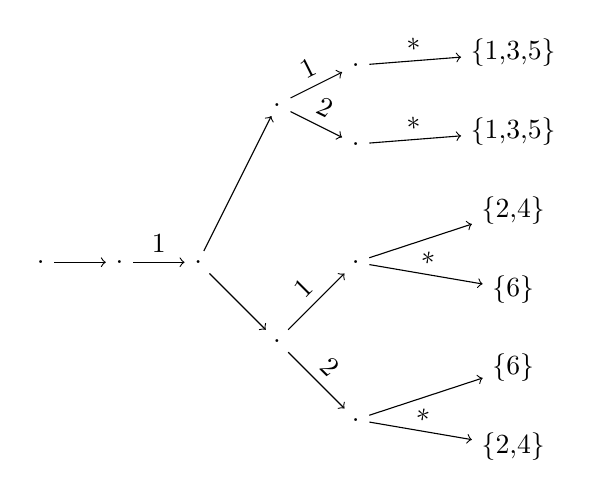
\begin{tikzpicture}[->,sloped,above]

	\node (root) at (0,2.5) {.};

	\node (h) at (1,2.5) {.};

	\node (h1) at (2,2.5) {.};

	\node (h1f) at (3,4.5) {.};
	\node (h1g) at (3,1.5) {.};

	\node (h1f1) at (4,5) {.};
	\node (h1f2) at (4,4) {.};
	\node (h1g1) at (4,2.5) {.};
	\node (h1g2) at (4,0.5) {.};

	\node (h1f1x) at (6,5) {\{1,3,5\}};
	\node (h1f2x) at (6,4) {\{1,3,5\}};
	\node (h1g1a) at (6,3) {\{2,4\}};
	\node (h1g1x) at (6,2) {\{6\}};
	\node (h1g2a) at (6,1) {\{6\}};
	\node (h1g2x) at (6,0) {\{2,4\}};

	\path (root) edge node {\( \mh \)} (h)
	(h) edge node {\( 1 \)} (h1)

	(h1)
	edge node {\( \mf \)} (h1f)
	edge node {\( \mg \)} (h1g)

	(h1f)
	edge node {\( 1 \)} (h1f1)
	edge node {\( 2 \)} (h1f2)

	(h1g)
	edge node {\( 1 \)} (h1g1)
	edge node {\( 2 \)} (h1g2)

	(h1f1)
	% edge node {\( \ma \)} (h1f1a)
	edge node {\( * \)} (h1f1x)

	(h1f2)
	%		edge node {\( \ma \)} (h1f2a)
	edge node {\( * \)} (h1f2x)


	(h1g1)
	edge node {\( \ma \)} (h1g1a)
	edge node {\( * \)} (h1g1x)

	(h1g2)
	edge node {\( \ma \)} (h1g2a)
	edge node {\( * \)} (h1g2x)
	;
	\end{tikzpicture}
\end{center}
\( \mh(\mg(y,x)) \mapsto \{ \mh.1.\mg.1.{*}, \mh.1.\mg.2.{*} \} \)
\end{example}

%+ PATH INDEXING/Retrieve
\begin{example}{Retrieve}
	\def\TRIEWIDTH{5cm}
	\def\TEXTWIDTH{\textwidth-\TRIEWIDTH-2em}

	\begin{minipage}{\TEXTWIDTH}
		\(
		\TI{t_1}\mh(\mf(x,y)),
		\TI{t_2}\mh(\mf({ x},{\ma})),
		\TI{t_3}\mh(\mf(\ma,\ma))
		 \)
		\begin{align*}
		\mh(\mf(z,\mb)) &\Rightarrow \{ \mh.1.\mf.1.{*}, \mh.1.\mf.2.\mb \}
		\\[0.7em]
		u : \mh(\mf({\colN z},{\colHi \mb}))
		& \mapsto
		{
			\{ t_1, {\colG t_2},
			{t_3} \}
		}
		{
			\cap \{t_1 \}
		}\\
%		{
			i : \mh(\mf(z, \mb)) &\mapsto \{ {\colG t_1,t_2,t_3 } \} \cap \{  \}
%		}
	\\
%		{
			g : \mh(\mf(z, \mb)) &\mapsto \{ t_1, {\colG t_2} \} \cap \{ t_1 \}
%		}
	\\
%		{
			v : \mh(\mf(z, \mb)) &\mapsto \{ {\colG t_1,t_2 }\} \cap \{  \}
%		}
	\\[0.7em]
%		{
			\colG v: \mh(\mf(z, z)) &\mapsto \{ {\colLo t_1},{\colG t_2} \} \cap \{ {\colLo t_1} \}
%		}
	\end{align*}
	\end{minipage}
	%
	\begin{minipage}{{\TRIEWIDTH}}
		\begin{tikzpicture}[->,dotted]
%		\ORIGIN

\def\pyL{-0.2}
\def\pxL{0.05}

\PAUSE

\node (root) at (2.5,5) {.};
\node (h) at (2.5,4) {.};
\path (root) edge node {$\mh$} (h);

\PAUSE
\node (h1) at (2.5,3) {.};
\path (h) edge node {$1$} (h1);

\PAUSE
\node (h1f) at (1.5,2) {.};
\path (h1) edge node {$\mf$} (h1f);

\PAUSE
\node (h1f1) at (0.5,1) {.};
\path (h1f) edge node {$1$} (h1f1);

\PAUSE
\node (h1f1x) at (0,0) {.};
\path (h1f1) edge node {$*$} (h1f1x);
\node (12) at (\pxL,\pyL) {\scriptsize$t_1,t_2$};

\PAUSE
\node (h1f1a) at (1,0) {.};
\path (h1f1) edge node {$\ma$} (h1f1a);
\node (3) at (\pxL+1,\pyL) {\scriptsize$t_3$};

\PAUSE
\node (h1f2) at (2.5,1) {.};
\path (h1f) edge node {$2$} (h1f2);

\PAUSE
\node (h1f2x) at (2,0) {.};
\path (h1f2) edge node {$*$} (h1f2x);
\node (1) at (\pxL+2,\pyL) {\scriptsize$t_1$};

\PAUSE
\node (h1f2a) at (3,0) {.};
\path (h1f2) edge node {$\ma$} (h1f2a);
\node (23) at (\pxL+3,\pyL) {\scriptsize$t_2,t_3$};


\node (lu) at (0,-0.5) {} ;
		\ORIGIN

\def\pyL{-0.2}
\def\pxL{0.05}

\node (root) at (2.5,5) {.};
\node (h) at (2.5,4) {.};
\path (root) edge node {$\mh$} (h);

\node (h1) at (2.5,3) {.};
\path (h) edge node {$1$} (h1);

\node (h1f) at (1.5,2) {.};
\path (h1) edge node {$\mf$} (h1f);

\node (h1f1) at (0.5,1) {.};
\path (h1f) edge node {$1$} (h1f1);

\node (h1f1x) at (0,0) {.};
\path (h1f1) edge node {$*$} (h1f1x);
\node (12) at (\pxL,\pyL) {\scriptsize$t_1,t_2$};

\node (h1f1a) at (1,0) {.};
\path (h1f1) edge node {$\ma$} (h1f1a);
\node (3) at (\pxL+1,\pyL) {\scriptsize$t_3$};

\node (h1f2) at (2.5,1) {.};
\path (h1f) edge node {$2$} (h1f2);

\node (h1f2x) at (2,0) {.};
\path (h1f2) edge node {$*$} (h1f2x);
\node (1) at (\pxL+2,\pyL) {\scriptsize$t_1$};

\node (h1f2a) at (3,0) {.};
\path (h1f2) edge node {$\ma$} (h1f2a);
\node (23) at (\pxL+3,\pyL) {\scriptsize$t_2,t_3$};

\node (lu) at (0,-0.5) {} ;

		\path[bend right, dashed, colN](root) edge (h);
		\node at (1.3,5) {\scriptsize\( (\mh,1.\mf.1.{*}) \)};
		\path[bend right, dashed, colN]	(h) edge (h1);
		\node at (1.0,4) {\scriptsize\( (1,\mf.1.{*}) \)};
		\path[bend right, dashed, colN]	(h1) edge (h1f);
		\node at (0.7,3) {\scriptsize\( (\mf,1.{*}) \)};
		\path[bend right, dashed, colN]	(h1f) edge (h1f1);
		\node at (0.4,2) {\scriptsize\( (1,{*}) \)};
		\path[bend right, dashed, colN]	(h1f1) edge (h1f1x)	;
		\node at (0.1,1) {\scriptsize\( ({*},\epsilon) \)};
		\path[bend right, dashed, colN]	(h1f1) edge (h1f1a);

		\path[bend left, dashed, colHi]	(root) edge (h)	;
		\node at (3.5,5) {\scriptsize\( (\mh,1.\mf.2.\mb) \)};
		\path[bend left, dashed, colHi]	(h) edge (h1)	;
		\node at (3.4,4) {\scriptsize\( (1,\mf.2.\mb) \)};
		\path[bend left, dashed, colHi]	(h1) edge (h1f)	;
		\node at (3.3,3) {\scriptsize\( (\mf,2.\mb) \)};
		\path[bend left, dashed, colHi]	(h1f) edge (h1f2)	;
		\node at (3.2,2) {\scriptsize\( (2,\mb) \)};
		\path[bend left, dashed, colHi]	(h1f2) edge (h1f2x)	;
		\node at (3.1,1) {\scriptsize\( (\mb,\epsilon) \)};
		\end{tikzpicture}
	\end{minipage}
\end{example}

%+ PATH INDEXING/Subterms
\begin{example}{Demodulation (Subterms)}

	\(
	\colG
	\TI{t_1}\mh(\mf(x,y)),
	\TI{t_2}\mh(\mf({ x},{\ma})),
	\TI{t_3}\mh(\mf(\ma,\ma)),
	\ldots,
%	\color{black}\mf(x,\ma) \foEQ x
	\color{black}\mf(x,\ma) \mEQ x
	 \)


	 \def\TRIEWIDTH{\textwidth/2-1em}% chktex 8
	 \def\TEXTWIDTH{\textwidth-\TRIEWIDTH-2em}
	\begin{minipage}{\TEXTWIDTH}
		\begin{tikzpicture}[->,dotted]
%		\ORIGIN

\def\pyL{-0.2}
\def\pxL{0.05}

\PAUSE

\node (root) at (2.5,5) {.};
\node (h) at (2.5,4) {.};
\path (root) edge node {$\mh$} (h);

\PAUSE
\node (h1) at (2.5,3) {.};
\path (h) edge node {$1$} (h1);

\PAUSE
\node (h1f) at (1.5,2) {.};
\path (h1) edge node {$\mf$} (h1f);

\PAUSE
\node (h1f1) at (0.5,1) {.};
\path (h1f) edge node {$1$} (h1f1);

\PAUSE
\node (h1f1x) at (0,0) {.};
\path (h1f1) edge node {$*$} (h1f1x);
\node (12) at (\pxL,\pyL) {\scriptsize$t_1,t_2$};

\PAUSE
\node (h1f1a) at (1,0) {.};
\path (h1f1) edge node {$\ma$} (h1f1a);
\node (3) at (\pxL+1,\pyL) {\scriptsize$t_3$};

\PAUSE
\node (h1f2) at (2.5,1) {.};
\path (h1f) edge node {$2$} (h1f2);

\PAUSE
\node (h1f2x) at (2,0) {.};
\path (h1f2) edge node {$*$} (h1f2x);
\node (1) at (\pxL+2,\pyL) {\scriptsize$t_1$};

\PAUSE
\node (h1f2a) at (3,0) {.};
\path (h1f2) edge node {$\ma$} (h1f2a);
\node (23) at (\pxL+3,\pyL) {\scriptsize$t_2,t_3$};


\node (lu) at (0,-0.5) {} ;
		\ORIGIN

\def\pyL{-0.2}
\def\pxL{0.05}

\node (root) at (2.5,5) {.};
\node (h) at (2.5,4) {.};
\path (root) edge node {$\mh$} (h);

\node (h1) at (2.5,3) {.};
\path (h) edge node {$1$} (h1);

\node (h1f) at (1.5,2) {.};
\path (h1) edge node {$\mf$} (h1f);

\node (h1f1) at (0.5,1) {.};
\path (h1f) edge node {$1$} (h1f1);

\node (h1f1x) at (0,0) {.};
\path (h1f1) edge node {$*$} (h1f1x);
\node (12) at (\pxL,\pyL) {\scriptsize$t_1,t_2$};

\node (h1f1a) at (1,0) {.};
\path (h1f1) edge node {$\ma$} (h1f1a);
\node (3) at (\pxL+1,\pyL) {\scriptsize$t_3$};

\node (h1f2) at (2.5,1) {.};
\path (h1f) edge node {$2$} (h1f2);

\node (h1f2x) at (2,0) {.};
\path (h1f2) edge node {$*$} (h1f2x);
\node (1) at (\pxL+2,\pyL) {\scriptsize$t_1$};

\node (h1f2a) at (3,0) {.};
\path (h1f2) edge node {$\ma$} (h1f2a);
\node (23) at (\pxL+3,\pyL) {\scriptsize$t_2,t_3$};

\node (lu) at (0,-0.5) {} ;

		\node (f) at (1.5,4) {.};
		\path[colN] (root) edge node {f} (f);

		\node (f1) at (0.5,4) {.};
		\path[colN] (f) edge node {1} (f1);

		\node (f1x) at (-0.5,4) {};
		\path[colN] (f1)	edge node {*} (f1x);

		\node[colN] (t1) at (-0.5,4.2) {\scriptsize\( t_1^1 \)};
		\node[colN] (t1) at (-0.5,3.8) {\scriptsize\(  t_2^1 \)};

		\node (f1a) at (-0.5,3) {};
		\path[colN] (f1) edge node {a} (f1a);

		\node[colN] (t3) at (-0.5,2.9) {\scriptsize\( t_3^1 \)};

		\node (f2) at (0.5,3) {.};
		\path[colN] (f) edge node {2}  (f2);

		\node (f2x) at (-0.5,2) {};
		\path[colN] (f2) edge node {*} (f2x);

		\node[colN] (t1) at (-0.5,1.9) {\scriptsize\( t_1^1 \)};

		\node (f2a) at (0.5,2) {};
		\path[colN] (f2) edge node {a} (f2a);

		\node[colN] (t2t3) at (0.5,1.9) {\scriptsize\( t_2^1,t_3^1 \)};

		\node (a) at (3.5,4) {};
		\path[colN] (root)  edge node {\( \ma \)} (a);
		\node[colN] (t2t3t3) at (3.5,3.9) {\scriptsize\( t_2^{12},t_3^{11,12} \)};

		\end{tikzpicture}
	\end{minipage}
	\hfill
	\begin{minipage}{{\TRIEWIDTH}}
		\def\pyL{-0.2}
		\def\pxL{0.05}
		\begin{tikzpicture}[->,dotted]
%		\ORIGIN

\def\pyL{-0.2}
\def\pxL{0.05}

\PAUSE

\node (root) at (2.5,5) {.};
\node (h) at (2.5,4) {.};
\path (root) edge node {$\mh$} (h);

\PAUSE
\node (h1) at (2.5,3) {.};
\path (h) edge node {$1$} (h1);

\PAUSE
\node (h1f) at (1.5,2) {.};
\path (h1) edge node {$\mf$} (h1f);

\PAUSE
\node (h1f1) at (0.5,1) {.};
\path (h1f) edge node {$1$} (h1f1);

\PAUSE
\node (h1f1x) at (0,0) {.};
\path (h1f1) edge node {$*$} (h1f1x);
\node (12) at (\pxL,\pyL) {\scriptsize$t_1,t_2$};

\PAUSE
\node (h1f1a) at (1,0) {.};
\path (h1f1) edge node {$\ma$} (h1f1a);
\node (3) at (\pxL+1,\pyL) {\scriptsize$t_3$};

\PAUSE
\node (h1f2) at (2.5,1) {.};
\path (h1f) edge node {$2$} (h1f2);

\PAUSE
\node (h1f2x) at (2,0) {.};
\path (h1f2) edge node {$*$} (h1f2x);
\node (1) at (\pxL+2,\pyL) {\scriptsize$t_1$};

\PAUSE
\node (h1f2a) at (3,0) {.};
\path (h1f2) edge node {$\ma$} (h1f2a);
\node (23) at (\pxL+3,\pyL) {\scriptsize$t_2,t_3$};


\node (lu) at (0,-0.5) {} ;
		\ORIGIN

\def\pyL{-0.2}
\def\pxL{0.05}

\node (root) at (2.5,5) {.};
\node (h) at (2.5,4) {.};
\path (root) edge node {$\mh$} (h);

\node (h1) at (2.5,3) {.};
\path (h) edge node {$1$} (h1);

\node (h1f) at (1.5,2) {.};
\path (h1) edge node {$\mf$} (h1f);

\node (h1f1) at (0.5,1) {.};
\path (h1f) edge node {$1$} (h1f1);

\node (h1f1x) at (0,0) {.};
\path (h1f1) edge node {$*$} (h1f1x);
\node (12) at (\pxL,\pyL) {\scriptsize$t_1,t_2$};

\node (h1f1a) at (1,0) {.};
\path (h1f1) edge node {$\ma$} (h1f1a);
\node (3) at (\pxL+1,\pyL) {\scriptsize$t_3$};

\node (h1f2) at (2.5,1) {.};
\path (h1f) edge node {$2$} (h1f2);

\node (h1f2x) at (2,0) {.};
\path (h1f2) edge node {$*$} (h1f2x);
\node (1) at (\pxL+2,\pyL) {\scriptsize$t_1$};

\node (h1f2a) at (3,0) {.};
\path (h1f2) edge node {$\ma$} (h1f2a);
\node (23) at (\pxL+3,\pyL) {\scriptsize$t_2,t_3$};

\node (lu) at (0,-0.5) {} ;

		\node[colN] (n-hsubs) at (5,4) {\( \mh \)};
		\path[dashdotted, above, pos=0.3,sloped,bend right=5,colN]  (n-hsubs) edge node {\scriptsize\( \ANGLES{\epsilon,\mh} \)} (h);

		\node[colN] (n-fsubs) at (5,3) {\( \mf \)};
		\path[dashdotted, above, pos=0.3,sloped, bend right=10,colN]  (n-fsubs) edge node {\scriptsize\( \ANGLES{1,\mf} \)} (h1f);

		\node[colN] (n-asubs) at (5,2) {\( \ma \)};
		\path[dashdotted, above, bend right, pos=0.3,sloped,colN]  (n-asubs) edge node {\scriptsize\( \ANGLES{11,\ma} \)} (h1f1a);
		\path[dashdotted, bend right, below, pos=0.3,sloped,colN]  (n-asubs) edge node {\scriptsize\( \ANGLES{12,\ma} \)} (h1f2a);

		\end{tikzpicture}
	\end{minipage}


\end{example}

%+ PATH INDEXING/SubtermTrees
\begin{example}{Subterm trees}
\begin{gather*}
\{
\TI{1}\mh(\mf(x,x)),
\TI{2}\mh(\mg(\ma,x)),
\TI{3}\mh(\mf(y,z))
\TI{4}\mh(\mg(\ma,y)),
\TI{5}\mh(\mf(y,x)),
\TI{6}\mh(\mg(y,a))
\}
\end{gather*}
%
\begin{center}
	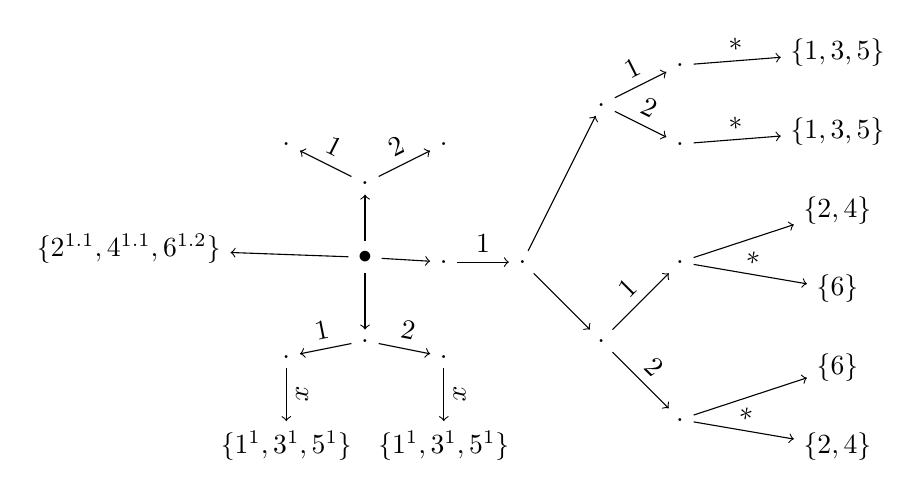
\begin{tikzpicture}[->,sloped,above]
	\node (root) at (0,2.5) {\( \bullet \)};
	%% right
	\node (h) at (1,2.5) {.};
	%
	\node (h1) at (2,2.5) {.};
	%
	\node (h1f) at (3,4.5) {.};
	\node (h1g) at (3,1.5) {.};
	%
	\node (h1f1) at (4,5) {.};
	\node (h1f2) at (4,4) {.};
	\node (h1g1) at (4,2.5) {.};
	\node (h1g2) at (4,0.5) {.};
	%
	\node (h1f1x) at (6,5) {\( \{1,3,5\} \)};
	\node (h1f2x) at (6,4) {\( \{1,3,5\} \)};
	\node (h1g1a) at (6,3) {\( \{2,4\} \)};
	\node (h1g1x) at (6,2) {\( \{6\} \)};
	\node (h1g2a) at (6,1) {\( \{6\} \)};
	\node (h1g2x) at (6,0) {\( \{2,4\} \)};
	%% down
	\node (f) at (0,1.5) {.};
	\node (f1) at (-1,1.3) {.};
	\node (f1x) at (-1,0) {\( \{1^{1},3^{1},5^{1}\} \)};
	\node (f2) at (1,1.3) {.};
	\node (f2x) at (1,0) {\( \{1^{1},3^{1},5^{1}\} \)};
	%% up
	\node (g) at (0,3.5) {.};
	\node (g1) at (-1,4) {.};
	\node (g2) at (1,4) {.};
	%% left
	\node (a) at (-3,2.5) {\( \{2^{1.1}, 4^{1.1}, 6^{1.2}\} \)};

	\path
	(root)
	edge node {\( \mh \)} (h)
	edge node {\( \mf \)} (f)
	edge node {\( \mg \)} (g)
	edge node {\( \ma \)} (a)

	(h) edge node {\( 1 \)} (h1)


	(h1)
	edge node {\( \mf \)} (h1f)
	edge node {\( \mg \)} (h1g)

	(h1f)
	edge node {\( 1 \)} (h1f1)
	edge node {\( 2 \)} (h1f2)

	(h1g)
	edge node {\( 1 \)} (h1g1)
	edge node {\( 2 \)} (h1g2)

	(h1f1)
	edge node {\( * \)} (h1f1x)

	(h1f2)
	edge node {\( * \)} (h1f2x)


	(h1g1)
	edge node {\( \ma \)} (h1g1a)
	edge node {\( * \)} (h1g1x)

	(h1g2)
	edge node {\( \ma \)} (h1g2a)
	edge node {\( * \)} (h1g2x)

	%
	(g) 	edge node {\( 1 \)} (g1)
	edge node {\( 2 \)} (g2)

	(f)	edge node {\( 1 \)} (f1)
	edge node {\( 2 \)} (f2)

	(f1)	edge node {\( x \)} (f1x)
	(f2)	edge node {\( x \)} (f2x)
	;


	\path (root)



	;

	\end{tikzpicture}
\end{center}
\end{example}





\subsection{Substitution Tree}
%% SUBSTITUTION TREES

%+ SUBSTITUTION TREES/Build+Index
\begin{example}{Substitution tree build}

	\(
	\TI{t_1}\mh(\mf(x,y)),
	\TI{t_2}\mh(\mf(x,\mh(\ma))),
	\TI{t_3}\mh(\mf(\mh(\ma),\ma)),
	\TI{t_4}\mh(\mf(\ma,\ma))
	 \)

	\begin{tikzpicture}[->]
%	\ORIGIN

\def\pyL{-0.2}
\def\pxL{0.05}

\PAUSE

\node (root) at (2.5,5) {.};
\node (h) at (2.5,4) {.};
\path (root) edge node {$\mh$} (h);

\PAUSE
\node (h1) at (2.5,3) {.};
\path (h) edge node {$1$} (h1);

\PAUSE
\node (h1f) at (1.5,2) {.};
\path (h1) edge node {$\mf$} (h1f);

\PAUSE
\node (h1f1) at (0.5,1) {.};
\path (h1f) edge node {$1$} (h1f1);

\PAUSE
\node (h1f1x) at (0,0) {.};
\path (h1f1) edge node {$*$} (h1f1x);
\node (12) at (\pxL,\pyL) {\scriptsize$t_1,t_2$};

\PAUSE
\node (h1f1a) at (1,0) {.};
\path (h1f1) edge node {$\ma$} (h1f1a);
\node (3) at (\pxL+1,\pyL) {\scriptsize$t_3$};

\PAUSE
\node (h1f2) at (2.5,1) {.};
\path (h1f) edge node {$2$} (h1f2);

\PAUSE
\node (h1f2x) at (2,0) {.};
\path (h1f2) edge node {$*$} (h1f2x);
\node (1) at (\pxL+2,\pyL) {\scriptsize$t_1$};

\PAUSE
\node (h1f2a) at (3,0) {.};
\path (h1f2) edge node {$\ma$} (h1f2a);
\node (23) at (\pxL+3,\pyL) {\scriptsize$t_2,t_3$};


\node (lu) at (0,-0.5) {} ;
	\ORIGIN


\node (root) at (0,0) {.};
\node (h) at (0,-1) {\( *_0 \mapsto \mh(*_1) \)};
\path (root) edge (h);

\node (f) at (0,-2) {\( *_1 \mapsto \mf(*_2,*_3) \)};
\path (h) edge (f);

\node (x2x) at (-2,-3) {\( *_2 \mapsto x \)} ;
\path (f) edge (x2x);

\node (x3y) at (-3,-4) {\( *_3 \mapsto y \)};
\path (x2x) edge (x3y);
\node (t1) at (-3,-4.4) {\( t_1 \)};

\node (x3ha) at (-1,-4) {\( *_3 \mapsto \mh(\ma) \)};
\path (x2x) edge (x3ha);
\node (t2) at (-1,-4.4) {\( t_2 \)};

\node (x3a)at (2,-3) {\( *_3\mapsto\ma \)};
\path (f) edge (x3a);

\node (x2ha) at (1,-4) {\( *_2\mapsto\mh(\ma) \)};
\path (x3a) edge (x2ha);
\node (t3) at (1,-4.4) {\( t_3 \)};

\node (x2a) at (3,-4) {\( *_2\mapsto\ma \)};
\path (x3a) edge (x2a);
\node (t4) at (3,-4.4) {\( t_4 \)};

	\end{tikzpicture}
\end{example}

%+ SUBSTITUTION TREES/Retrieve+Index
\begin{example}{Substitution tree retrieve}

	\(
	\TI{t_1}\mh(\mf(x,y)),
	\TI{t_2}\mh(\mf(x,\mh(\ma))),
	\TI{t_3}\mh(\mf(\mh(\ma),\ma)),
	\TI{t_4}\mh(\mf(\ma,\ma))
	 \)

	\begin{tikzpicture}[->]
%	\ORIGIN

\def\pyL{-0.2}
\def\pxL{0.05}

\PAUSE

\node (root) at (2.5,5) {.};
\node (h) at (2.5,4) {.};
\path (root) edge node {$\mh$} (h);

\PAUSE
\node (h1) at (2.5,3) {.};
\path (h) edge node {$1$} (h1);

\PAUSE
\node (h1f) at (1.5,2) {.};
\path (h1) edge node {$\mf$} (h1f);

\PAUSE
\node (h1f1) at (0.5,1) {.};
\path (h1f) edge node {$1$} (h1f1);

\PAUSE
\node (h1f1x) at (0,0) {.};
\path (h1f1) edge node {$*$} (h1f1x);
\node (12) at (\pxL,\pyL) {\scriptsize$t_1,t_2$};

\PAUSE
\node (h1f1a) at (1,0) {.};
\path (h1f1) edge node {$\ma$} (h1f1a);
\node (3) at (\pxL+1,\pyL) {\scriptsize$t_3$};

\PAUSE
\node (h1f2) at (2.5,1) {.};
\path (h1f) edge node {$2$} (h1f2);

\PAUSE
\node (h1f2x) at (2,0) {.};
\path (h1f2) edge node {$*$} (h1f2x);
\node (1) at (\pxL+2,\pyL) {\scriptsize$t_1$};

\PAUSE
\node (h1f2a) at (3,0) {.};
\path (h1f2) edge node {$\ma$} (h1f2a);
\node (23) at (\pxL+3,\pyL) {\scriptsize$t_2,t_3$};


\node (lu) at (0,-0.5) {} ;
	\ORIGIN


\node (root) at (0,0) {.};
\node (h) at (0,-1) {\( *_0 \mapsto \mh(*_1) \)};
\path (root) edge (h);

\node (f) at (0,-2) {\( *_1 \mapsto \mf(*_2,*_3) \)};
\path (h) edge (f);

\node (x2x) at (-2,-3) {\( *_2 \mapsto x \)} ;
\path (f) edge (x2x);

\node (x3y) at (-3,-4) {\( *_3 \mapsto y \)};
\path (x2x) edge (x3y);
\node (t1) at (-3,-4.4) {\( t_1 \)};

\node (x3ha) at (-1,-4) {\( *_3 \mapsto \mh(\ma) \)};
\path (x2x) edge (x3ha);
\node (t2) at (-1,-4.4) {\( t_2 \)};

\node (x3a)at (2,-3) {\( *_3\mapsto\ma \)};
\path (f) edge (x3a);

\node (x2ha) at (1,-4) {\( *_2\mapsto\mh(\ma) \)};
\path (x3a) edge (x2ha);
\node (t3) at (1,-4.4) {\( t_3 \)};

\node (x2a) at (3,-4) {\( *_2\mapsto\ma \)};
\path (x3a) edge (x2a);
\node (t4) at (3,-4.4) {\( t_4 \)};
	\end{tikzpicture}
\end{example}

%% DISCRIMINATION TREE
\subsection{Discrimination Tree}

%\ORIGIN

\node (root) at (1,0) {.};
\node (h) at (0,-1) {.};
\path (root) edge node {\( \mh \)} (h);
\node (hf) at (-1,-2) {.};
\path (h) edge node {\( \mf \)} (hf);
\node (hfx) at (-2,-3) {.};
\path (hf) edge node {\( * \)} (hfx);
\node (n-hfxx) at (-3,-4) {.};
\path (hfx) edge node {\( * \)} (n-hfxx);
\node (1) at (-3,-4.2) {\scriptsize \( t_1 \)};

\node (n-hfxh) at (-2,-4) {.};
\path (hfx) edge node {\( \mh \)} (n-hfxh);
\node (n-hfxha) at (-2,-5) {.};
\path (n-hfxh) edge node {\( \ma \)} (n-hfxha);
\node (2) at (-2,-5.2) {\scriptsize \( t_2 \)};

\node (hfh) at (-1,-3) {.};
\path (hf) edge node {\( \mh \)} (hfh);
\node (n-hfha) at (-1,-4) {.};
\path (hfh) edge node {\( \ma \)} (n-hfha);
\path[dashdotted,bend left=45,gray] (hf) edge (n-hfha);
\node (n-hfhaa) at (-1,-5) {.};
\path (n-hfha) edge node {\( \ma \)} (n-hfhaa);
\node (3) at (-1,-5.2) {\scriptsize \( t_3 \)};
%\(
\TI{t_1}\mh(\mf(x,y)),
\TI{t_2}\mh(\mf(x,\mh(\ma))),
\TI{t_3}\mh(\mf(\mh(\ma),\ma))
\)
%% DISCRIMINATION TREE/Build+Terms+Index
\begin{example}{Build}

	\def\TRIEWIDTH{4.4cm}
	\def\TEXTWIDTH{\textwidth-\TRIEWIDTH-2em}
	\begin{minipage}{\TEXTWIDTH}
%		$
\TI{\ell_1}\mP(\mf(x,y)), 
\TI{\ell_2}\mP(\mf(x,\mh(\ma))),
\TI{\ell_3}\mP(\mf(\mh(\ma),\ma))
$
		\(
\TI{t_1}\mh(\mf(x,y)),
\TI{t_2}\mh(\mf(x,\mh(\ma))),
\TI{t_3}\mh(\mf(\mh(\ma),\ma))
\)
		\begin{align*}
		t_1 &\Rightarrow \mh.\mf.{*}.{*}\\
		t_2 &\Rightarrow \mh.\mf.{*}.\mh.\ma \\
		t_3 &\Rightarrow \mh.\mf.\mh.\ma.\ma
		\end{align*}
	\end{minipage}
	\begin{minipage}{\TRIEWIDTH}
		\def\pyL{-0.3}
		\def\pxL{-0.0}
		\begin{tikzpicture}[->,dotted]
%		\ORIGIN

\def\pyL{-0.2}
\def\pxL{0.05}

\PAUSE

\node (root) at (2.5,5) {.};
\node (h) at (2.5,4) {.};
\path (root) edge node {$\mh$} (h);

\PAUSE
\node (h1) at (2.5,3) {.};
\path (h) edge node {$1$} (h1);

\PAUSE
\node (h1f) at (1.5,2) {.};
\path (h1) edge node {$\mf$} (h1f);

\PAUSE
\node (h1f1) at (0.5,1) {.};
\path (h1f) edge node {$1$} (h1f1);

\PAUSE
\node (h1f1x) at (0,0) {.};
\path (h1f1) edge node {$*$} (h1f1x);
\node (12) at (\pxL,\pyL) {\scriptsize$t_1,t_2$};

\PAUSE
\node (h1f1a) at (1,0) {.};
\path (h1f1) edge node {$\ma$} (h1f1a);
\node (3) at (\pxL+1,\pyL) {\scriptsize$t_3$};

\PAUSE
\node (h1f2) at (2.5,1) {.};
\path (h1f) edge node {$2$} (h1f2);

\PAUSE
\node (h1f2x) at (2,0) {.};
\path (h1f2) edge node {$*$} (h1f2x);
\node (1) at (\pxL+2,\pyL) {\scriptsize$t_1$};

\PAUSE
\node (h1f2a) at (3,0) {.};
\path (h1f2) edge node {$\ma$} (h1f2a);
\node (23) at (\pxL+3,\pyL) {\scriptsize$t_2,t_3$};


\node (lu) at (0,-0.5) {} ;
		\ORIGIN

\node (root) at (1,0) {.};
\node (h) at (0,-1) {.};
\path (root) edge node {\( \mh \)} (h);
\node (hf) at (-1,-2) {.};
\path (h) edge node {\( \mf \)} (hf);
\node (hfx) at (-2,-3) {.};
\path (hf) edge node {\( * \)} (hfx);
\node (n-hfxx) at (-3,-4) {.};
\path (hfx) edge node {\( * \)} (n-hfxx);
\node (1) at (-3,-4.2) {\scriptsize \( t_1 \)};

\node (n-hfxh) at (-2,-4) {.};
\path (hfx) edge node {\( \mh \)} (n-hfxh);
\node (n-hfxha) at (-2,-5) {.};
\path (n-hfxh) edge node {\( \ma \)} (n-hfxha);
\node (2) at (-2,-5.2) {\scriptsize \( t_2 \)};

\node (hfh) at (-1,-3) {.};
\path (hf) edge node {\( \mh \)} (hfh);
\node (n-hfha) at (-1,-4) {.};
\path (hfh) edge node {\( \ma \)} (n-hfha);
\path[dashdotted,bend left=45,gray] (hf) edge (n-hfha);
\node (n-hfhaa) at (-1,-5) {.};
\path (n-hfha) edge node {\( \ma \)} (n-hfhaa);
\node (3) at (-1,-5.2) {\scriptsize \( t_3 \)};
		\node (lu) at (-3,-5.5) {} ;
		\end{tikzpicture}
	\end{minipage}
	%
\end{example}



%% DISCRIMINATION TREE/Index
%% DISCRIMINATION TREE/IndexEdges

%+ DISCRIMINATION TREE/Retrieve+Terms+Index
\begin{example}{Retrieve}

	\def\TRIEWIDTH{4.4cm}
	\def\TEXTWIDTH{\textwidth-\TRIEWIDTH-2em}
	\begin{minipage}{\TEXTWIDTH}
%		$
\TI{\ell_1}\mP(\mf(x,y)), 
\TI{\ell_2}\mP(\mf(x,\mh(\ma))),
\TI{\ell_3}\mP(\mf(\mh(\ma),\ma))
$
		\(
\TI{t_1}\mh(\mf(x,y)),
\TI{t_2}\mh(\mf(x,\mh(\ma))),
\TI{t_3}\mh(\mf(\mh(\ma),\ma))
\)
		\begin{align*}
		\mh(\mf(x',\ma))&\Rightarrow \mh.\mf.{*}.\ma
		\\[0.7em]
		u: \mh(\mf(x',\ma))&\mapsto \{
		{t_1,}
		{t_3}
		\}
		\\
					i:\mh(\mf(x',\ma))&\mapsto \{t_3\}  \\
					g:\mh(\mf(x',\ma))&\mapsto \{t_1\} \\
					v:\mh(\mf(x',\ma))&\mapsto \{  \} \\
		\end{align*}
	\end{minipage}
%
	\begin{minipage}{\TRIEWIDTH}
		\begin{tikzpicture}[->,dotted]
%		\ORIGIN

\def\pyL{-0.2}
\def\pxL{0.05}

\PAUSE

\node (root) at (2.5,5) {.};
\node (h) at (2.5,4) {.};
\path (root) edge node {$\mh$} (h);

\PAUSE
\node (h1) at (2.5,3) {.};
\path (h) edge node {$1$} (h1);

\PAUSE
\node (h1f) at (1.5,2) {.};
\path (h1) edge node {$\mf$} (h1f);

\PAUSE
\node (h1f1) at (0.5,1) {.};
\path (h1f) edge node {$1$} (h1f1);

\PAUSE
\node (h1f1x) at (0,0) {.};
\path (h1f1) edge node {$*$} (h1f1x);
\node (12) at (\pxL,\pyL) {\scriptsize$t_1,t_2$};

\PAUSE
\node (h1f1a) at (1,0) {.};
\path (h1f1) edge node {$\ma$} (h1f1a);
\node (3) at (\pxL+1,\pyL) {\scriptsize$t_3$};

\PAUSE
\node (h1f2) at (2.5,1) {.};
\path (h1f) edge node {$2$} (h1f2);

\PAUSE
\node (h1f2x) at (2,0) {.};
\path (h1f2) edge node {$*$} (h1f2x);
\node (1) at (\pxL+2,\pyL) {\scriptsize$t_1$};

\PAUSE
\node (h1f2a) at (3,0) {.};
\path (h1f2) edge node {$\ma$} (h1f2a);
\node (23) at (\pxL+3,\pyL) {\scriptsize$t_2,t_3$};


\node (lu) at (0,-0.5) {} ;
		\ORIGIN

\node (root) at (1,0) {.};
\node (h) at (0,-1) {.};
\path (root) edge node {\( \mh \)} (h);
\node (hf) at (-1,-2) {.};
\path (h) edge node {\( \mf \)} (hf);
\node (hfx) at (-2,-3) {.};
\path (hf) edge node {\( * \)} (hfx);
\node (n-hfxx) at (-3,-4) {.};
\path (hfx) edge node {\( * \)} (n-hfxx);
\node (1) at (-3,-4.2) {\scriptsize \( t_1 \)};

\node (n-hfxh) at (-2,-4) {.};
\path (hfx) edge node {\( \mh \)} (n-hfxh);
\node (n-hfxha) at (-2,-5) {.};
\path (n-hfxh) edge node {\( \ma \)} (n-hfxha);
\node (2) at (-2,-5.2) {\scriptsize \( t_2 \)};

\node (hfh) at (-1,-3) {.};
\path (hf) edge node {\( \mh \)} (hfh);
\node (n-hfha) at (-1,-4) {.};
\path (hfh) edge node {\( \ma \)} (n-hfha);
\path[dashdotted,bend left=45,gray] (hf) edge (n-hfha);
\node (n-hfhaa) at (-1,-5) {.};
\path (n-hfha) edge node {\( \ma \)} (n-hfhaa);
\node (3) at (-1,-5.2) {\scriptsize \( t_3 \)};
		\path[bend right, dashed, colN] (root) edge  (h);
		\path[bend right, dashed, colN] (h) edge  (hf);
		\path[bend right, dashed, colN] (hf) edge (hfx);
		\path[bend right, dashed, colN] (hfx) edge  (n-hfxx);
		\path[bend right, dashed, colN] (hf) edge  (n-hfha);
		\path[bend right, dashed, colN] (n-hfha) edge (n-hfhaa);

		\node (lu) at (-3,-5.5) {} ;
		\end{tikzpicture}
	\end{minipage}
	%
\end{example}

%% DISCRIMINATION TREE/Subterms+Terms+Index
\begin{example}{Subterms}
	\def\TRIEWIDTH{\textwidth/2-1em}% chktex 8
%%	$
\TI{\ell_1}\mP(\mf(x,y)), 
\TI{\ell_2}\mP(\mf(x,\mh(\ma))),
\TI{\ell_3}\mP(\mf(\mh(\ma),\ma))
$
	\(
\TI{t_1}\mh(\mf(x,y)),
\TI{t_2}\mh(\mf(x,\mh(\ma))),
\TI{t_3}\mh(\mf(\mh(\ma),\ma))
\)
%	\vspace{1em}

	\begin{minipage}{\TRIEWIDTH}
		\begin{tikzpicture}[->, dotted]
%		\ORIGIN

\def\pyL{-0.2}
\def\pxL{0.05}

\PAUSE

\node (root) at (2.5,5) {.};
\node (h) at (2.5,4) {.};
\path (root) edge node {$\mh$} (h);

\PAUSE
\node (h1) at (2.5,3) {.};
\path (h) edge node {$1$} (h1);

\PAUSE
\node (h1f) at (1.5,2) {.};
\path (h1) edge node {$\mf$} (h1f);

\PAUSE
\node (h1f1) at (0.5,1) {.};
\path (h1f) edge node {$1$} (h1f1);

\PAUSE
\node (h1f1x) at (0,0) {.};
\path (h1f1) edge node {$*$} (h1f1x);
\node (12) at (\pxL,\pyL) {\scriptsize$t_1,t_2$};

\PAUSE
\node (h1f1a) at (1,0) {.};
\path (h1f1) edge node {$\ma$} (h1f1a);
\node (3) at (\pxL+1,\pyL) {\scriptsize$t_3$};

\PAUSE
\node (h1f2) at (2.5,1) {.};
\path (h1f) edge node {$2$} (h1f2);

\PAUSE
\node (h1f2x) at (2,0) {.};
\path (h1f2) edge node {$*$} (h1f2x);
\node (1) at (\pxL+2,\pyL) {\scriptsize$t_1$};

\PAUSE
\node (h1f2a) at (3,0) {.};
\path (h1f2) edge node {$\ma$} (h1f2a);
\node (23) at (\pxL+3,\pyL) {\scriptsize$t_2,t_3$};


\node (lu) at (0,-0.5) {} ;
		\ORIGIN

\node (root) at (1,0) {.};
\node (h) at (0,-1) {.};
\path (root) edge node {\( \mh \)} (h);
\node (hf) at (-1,-2) {.};
\path (h) edge node {\( \mf \)} (hf);
\node (hfx) at (-2,-3) {.};
\path (hf) edge node {\( * \)} (hfx);
\node (n-hfxx) at (-3,-4) {.};
\path (hfx) edge node {\( * \)} (n-hfxx);
\node (1) at (-3,-4.2) {\scriptsize \( t_1 \)};

\node (n-hfxh) at (-2,-4) {.};
\path (hfx) edge node {\( \mh \)} (n-hfxh);
\node (n-hfxha) at (-2,-5) {.};
\path (n-hfxh) edge node {\( \ma \)} (n-hfxha);
\node (2) at (-2,-5.2) {\scriptsize \( t_2 \)};

\node (hfh) at (-1,-3) {.};
\path (hf) edge node {\( \mh \)} (hfh);
\node (n-hfha) at (-1,-4) {.};
\path (hfh) edge node {\( \ma \)} (n-hfha);
\path[dashdotted,bend left=45,gray] (hf) edge (n-hfha);
\node (n-hfhaa) at (-1,-5) {.};
\path (n-hfha) edge node {\( \ma \)} (n-hfhaa);
\node (3) at (-1,-5.2) {\scriptsize \( t_3 \)};
		\node (ha) at (1,-2) {.} ;
		\path[dashdotted,colN] (h) edge node {\( \ma \)} (ha);
		\node (tha)  at (1,-2.2) {\scriptsize\( t_2^{{\colN 12}}, t_3^{{\colN 111}} \)} ;
		{(lu) at (-3.5,-5.5) {+}}

		\end{tikzpicture}
	\end{minipage}
%	\hfill{
		\begin{minipage}{\TRIEWIDTH}
			\begin{tikzpicture}[->,dotted]
%
%%			\ORIGIN

\def\pyL{-0.2}
\def\pxL{0.05}

\PAUSE

\node (root) at (2.5,5) {.};
\node (h) at (2.5,4) {.};
\path (root) edge node {$\mh$} (h);

\PAUSE
\node (h1) at (2.5,3) {.};
\path (h) edge node {$1$} (h1);

\PAUSE
\node (h1f) at (1.5,2) {.};
\path (h1) edge node {$\mf$} (h1f);

\PAUSE
\node (h1f1) at (0.5,1) {.};
\path (h1f) edge node {$1$} (h1f1);

\PAUSE
\node (h1f1x) at (0,0) {.};
\path (h1f1) edge node {$*$} (h1f1x);
\node (12) at (\pxL,\pyL) {\scriptsize$t_1,t_2$};

\PAUSE
\node (h1f1a) at (1,0) {.};
\path (h1f1) edge node {$\ma$} (h1f1a);
\node (3) at (\pxL+1,\pyL) {\scriptsize$t_3$};

\PAUSE
\node (h1f2) at (2.5,1) {.};
\path (h1f) edge node {$2$} (h1f2);

\PAUSE
\node (h1f2x) at (2,0) {.};
\path (h1f2) edge node {$*$} (h1f2x);
\node (1) at (\pxL+2,\pyL) {\scriptsize$t_1$};

\PAUSE
\node (h1f2a) at (3,0) {.};
\path (h1f2) edge node {$\ma$} (h1f2a);
\node (23) at (\pxL+3,\pyL) {\scriptsize$t_2,t_3$};


\node (lu) at (0,-0.5) {} ;
			\ORIGIN

\node (root) at (1,0) {.};
\node (h) at (0,-1) {.};
\path (root) edge node {\( \mh \)} (h);
\node (hf) at (-1,-2) {.};
\path (h) edge node {\( \mf \)} (hf);
\node (hfx) at (-2,-3) {.};
\path (hf) edge node {\( * \)} (hfx);
\node (n-hfxx) at (-3,-4) {.};
\path (hfx) edge node {\( * \)} (n-hfxx);
\node (1) at (-3,-4.2) {\scriptsize \( t_1 \)};

\node (n-hfxh) at (-2,-4) {.};
\path (hfx) edge node {\( \mh \)} (n-hfxh);
\node (n-hfxha) at (-2,-5) {.};
\path (n-hfxh) edge node {\( \ma \)} (n-hfxha);
\node (2) at (-2,-5.2) {\scriptsize \( t_2 \)};

\node (hfh) at (-1,-3) {.};
\path (hf) edge node {\( \mh \)} (hfh);
\node (n-hfha) at (-1,-4) {.};
\path (hfh) edge node {\( \ma \)} (n-hfha);
\path[dashdotted,bend left=45,gray] (hf) edge (n-hfha);
\node (n-hfhaa) at (-1,-5) {.};
\path (n-hfha) edge node {\( \ma \)} (n-hfhaa);
\node (3) at (-1,-5.2) {\scriptsize \( t_3 \)};
			\node (n-hsubs) at (1,-4.5) {};
			\path[dashdotted, colN, sloped,above] (n-hsubs)
			edge[pos=0.4] node[sloped]
			{\scriptsize\( \ANGLES{\epsilon,\mh} \)}  (h);
			\path[dashdotted, colN,sloped, above] (n-hsubs)
			edge[bend left=0,pos=0.4,sloped]
			node
			{\scriptsize\( \ANGLES{11,\mh} \)}
			(hfh);
%
			\path[dashdotted, colN] (n-hsubs)
			edge[bend left=0,pos=0.2,sloped]
			node[below] {\scriptsize \( \ANGLES{12,\mh} \)}
			(n-hfxh);
%
			\node (lu) at (-3.5,-5.5) {} ;
			\end{tikzpicture}
	\end{minipage}
%	%
\end{example}






